\documentclass{article}
\usepackage{pdfpages}

\author{Yeoun Chan Kim \and John Strauser \and Xuanang Wang}

\title{CS440 Assignment2}

\begin{document}

\maketitle

\section*{P1}

\hspace{5mm}


A) 	

        All five True = P(A,B,C,D,E) = P(A)P(B)P(C)P(D$|$A+B)P(E$|$B+C)

	P(A) = 0.2
	
	P(B) = 0.5
	
	P(C) = 0.8
	
	P(D$|$A+B) = 0.1
	
	P(E$|$B+C) = 0.3
	
	P(A,B,C,D,E) = 0.2*0.5*0.8*0.1*0.3 = 0.0024

\hspace{5mm}

B)	

        All five false = P(!A,!B,!C,!D,!E) = P(!A)P(!B)P(!C)P(!D$|$!A+!B)P(!E$|$!B+!C)
        
	P(!A) = 0.8
	
	P(!B) = 0.5
	
	P(!C) = 0.2
	
	P(!D$|$!A+!B) = 0.1
	
	P(!E$|$!B+!C) = 0.8
	
	P(!A,!B,!C,!D,!E) = 0.8*0.5*0.2*0.1*0.8 = 0.0064

\hspace{5mm}

C)	

        P(!A$|$B+C+D+E) = P(!A+B+C+D+E) / P(B+C+D+E)

	P(!A+B+C+D+E) = P(!A)P(B)P(C)P(D$|$!A+B)P(E$|$B+C) = 0.8*0.5*0.8*0.6*0.3 = 0.0576
	
	P(B+C+D+E) =  P(A,B,C,D,E) + P(!A,B,C,D,E) = 0.0024 + 0.0576 = 0.06
	
	P(!A$|$B+C+D+E) = 0.0576 / 0.06 = 0.96
	
	
\section*{P2}

\hspace{5mm}

A) 	

        P(Burglary$|$JohnCalls + MaryCalls) = P(B,J,M,A,E) + P(B,J,M,A,!E) + P(B,J,M,!A,E) + P(B,J,M,!A,!E) / P(B,J,M) + P(!B,J,M)

	P(B,J,M,A,E) = P(B)P(J$|$A)P(M$|$A)P(A$|$B+E)P(E) = 0.001*0.9*0.7*0.95*0.002 = 0.000001197
	
	P(B,J,M,A,!E) = P(B)P(J$|$A)P(M$|$A)P(A$|$B+!E)P(!E) = 0.001*0.9*0.7*0.94*0.998 = 0.000591
	
	P(B,J,M,!A,E) = P(B)P(J$|$!A)P(M$|$!A)P(-A$|$B+E)P(E) = 0.001*0.05*0.01*0.05*0.002 = 0.000000000005
	
	P(B,J,M,!A,!E) = P(B)P(J$|$!A)P(M$|$!A)P(!A$|$B+!E)P(!E) = 0.001*0.05*0.01*0.06*0.998 = 0.0000000299
	
	P(B,J,M) = P(B,J,M,A,E) + P(B,J,M,A,!E) + P(B,J,M,!A,E) + P(B,J,M,!A,!E) = 0.000001197 + 0.000591 + 0.000000000005 + 0.0000000299 = 0.000592
	
	P(!B,J,M) = P(!B,J,M,A,E) + P(!B,J,M,A,!E) + P(!B,J,M,!A,E) + P(!B,J,M,!A,!E)
	
	P(!B,J,M,A,E) = P(!B)P(J$|$A)P(M$|$A)P(A$|$!B+E)P(E) = 0.999 * 0.9 * 0.7 * 0.29 * 0.002 = 0.000365
	
	P(!B,J,M,A,!E) = P(!B)P(J$|$A)P(M$|$A)P(A$|$!B+!E)P(!E) = 0.999 * 0.9 * 0.7 * 0.001 * 0.998 = 0.000628
	
	P(!B,J,M,!A,E) = P(!B)P(J$|$!A)P(M$|$!A)P(!A$|$!B+E)P(E) = 0.999 * 0.05 * 0.01 * 0.71 * 0.002 = 0.000000709
	
	P(!B,J,M,!A,!E) = P(!B)P(J$|$!A)P(M$|$!A)P(!A$|$!B+!E)P(!E) = 0.999 * 0.05 * 0.01 * 0.999 * 0.998 = 0.000498
	
	P(!B,J,M) = 0.000365 + 0.000628 + 0.000000709 + 0.000498 = 0.00149
	
	P(Burglary$|$JohnCalls + MaryCalls) = (0.000592)/(0.000592 + 0.00149) = 0.284
	
\hspace{5mm}
	
B)	
        enumeration tree would be a straight line. Therefore worst case is that all n variables must be checked. 

	complexity using enumeration = O(n)
	
	complexity using variable elimination = O(n)
	
\section*{P3}

\hspace{5mm}

A)

OC : card holder owns a computer or smart phone.

Fraud : current transaction is fraudulent.

Trav : card holder is currently travelling.

FP : current transaction is a foreign purchase.

IP : current purchase is an internet purchase.

CRP : a computer related purchase was made in the past week

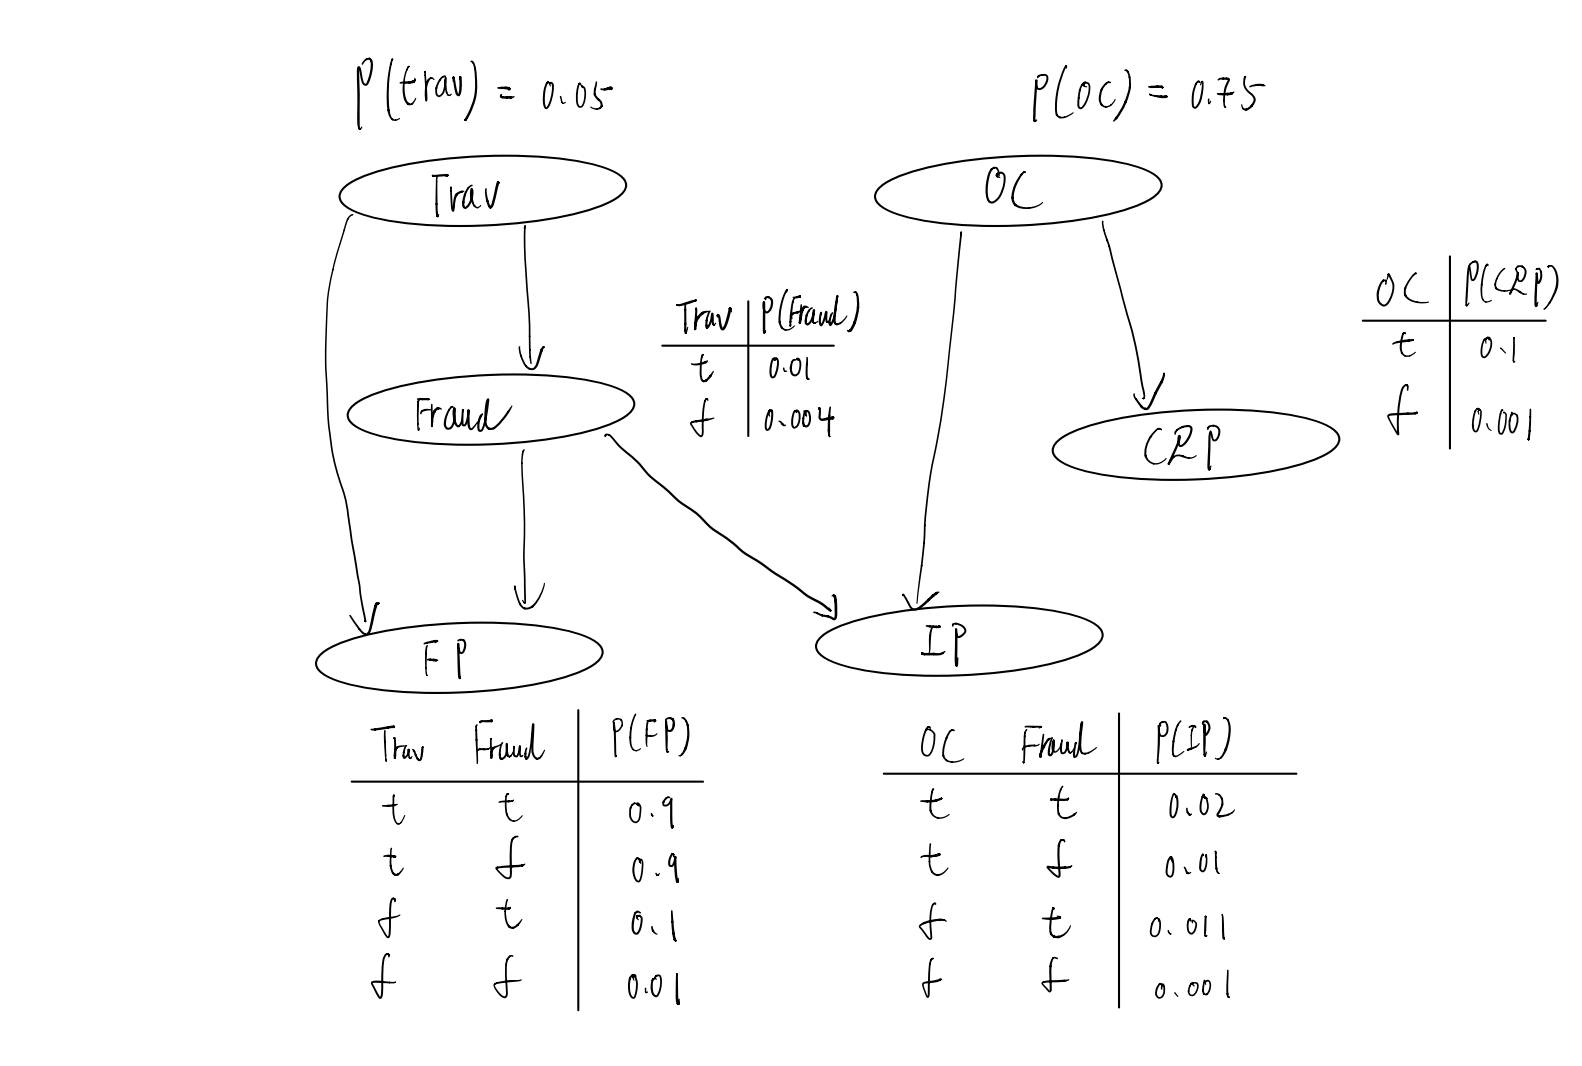
\includepdf[pages=-]{graph.png}


B)

	P(Fraud) = (P(Fraud + Trav) + P(Fraud + !Trav)) / (P(Fraud) + P(!Fraud))
	
	P(Fraud) = (P(Fraud$|$Trav)P(Trav) + P(Fraud$|$!Trav)P(!Trav)) / (1)
	
	P(Fraud) = 0.01*0.05 + 0.004*0.95
	
	P(Fraud) = 0.0043
	
	P(Fraud $|$ FP + !IP + CRP) = (P(Fraud + FP + !IP + CRP + Trav + OC) + P(Fraud + FP + !IP + CRP + Trav + !OC) + P(Fraud + FP + !IP + CRP + !Trav + OC) + P(Fraud + FP + !IP + CRP + !Trav + !OC))/(P(Fraud + FP + !IP + CRP) + P(!Fraud + FP + !IP + CRP + Trav + OC))
	
        P(Fraud + FP + !IP + CRP + Trav + OC) = P(Fraud$|$Trav)P(FP$|$Trav+Fraud)\\P(!IP$|$OC+Fraud)P(CRP$|$OC)P(Trav)P(OC)\\ = 0.01 * 0.9 * 0.98 * 0.1 * 0.05 * 0.75\\ = 0.00003308
	
	P(Fraud + FP + !IP + CRP + Trav + !OC) = P(Fraud$|$Trav)P(FP$|$Trav+Fraud)\\P(!IP$|$!OC+Fraud)P(CRP$|$!OC)P(Trav)P(!OC)\\ = 0.01 * 0.9 * 0.989 * 0.001 * 0.05 * 0.25 = 0.0000001112
	
	P(Fraud + FP + !IP + CRP + !Trav + OC) = P(Fraud$|$!Trav)P(FP$|$!Trav+Fraud)\\P(!IP$|$OC+Fraud)P(CRP$|$OC)P(!Trav)P(OC)\\ = 0.004 * 0.1 * 0.98 * 0.1 * 0.95 * 0.75 = 0.00002793
	
	P(Fraud + FP + !IP + CRP + !Trav + !OC) = P(Fraud$|$!Trav)P(FP$|$!Trav+Fraud)\\P(!IP$|$!OC+Fraud)P(CRP$|$!OC)P(!Trav)P(!OC)\\ = 0.004 * 0.1 * 0.989 * 0.001 * 0.95 * 0.25 = 0.000000093955
	
	P(Fraud + FP + !IP + CRP) = P(Fraud + FP + !IP + CRP + Trav + OC) + P(Fraud + FP + !IP + CRP + Trav + !OC) + P(Fraud + FP + !IP + CRP + !Trav + OC) + P(Fraud + FP + !IP + CRP + !Trav + !OC)\\ = 0.00003308 + 0.0000001112 + 0.00002793 + 0.000000093955 = 0.000061215155
		
	P(!Fraud + FP + !IP + CRP) = P(!Fraud + FP + !IP + CRP + Trav + OC) + P(!Fraud + FP + !IP + CRP + Trav + !OC) + P(!Fraud + FP + !IP + CRP + !Trav + OC) + P(!Fraud + FP + !IP + CRP + !Trav + !OC)
	
	P(!Fraud + FP + !IP + CRP + Trav + OC) = P(!Fraud$|$Trav)P(FP$|$Trav+!Fraud)\\P(!IP$|$OC+!Fraud)P(CRP$|$OC)P(Trav)P(OC)\\= 0.99 * 0.9 * 0.99 * 0.1 * 0.05 * 0.75 = 0.0033078375
	
	P(!Fraud + FP + !IP + CRP + Trav + !OC) = P(!Fraud$|$Trav)P(FP$|$Trav+!Fraud)\\P(!IP$|$!OC+!Fraud)P(CRP$|$!OC)P(Trav)P(!OC)\\ = 0.99 * 0.9 * 0.999 * 0.001 * 0.05 * 0.25 = 0.000011126
	
	P(!Fraud + FP + !IP + CRP + !Trav + OC) = P(!Fraud$|$!Trav)P(FP$|$!Trav+!Fraud)\\P(!IP$|$OC+!Fraud)P(CRP$|$OC)P(!Trav)P(OC)\\ = 0.996 * 0.01 * 0.99 * 0.1 * 0.95 * 0.75 = 0.00070255
	
	P(!Fraud + FP + !IP + CRP + !Trav + !OC) = P(!Fraud$|$!Trav)P(FP$|$!Trav+!Fraud)\\P(!IP$|$!OC+!Fraud)P(CRP$|$!OC)P(!Trav)P(!OC)\\ = 0.996 * 0.01 * 0.999 * 0.001 * 0.95 * 0.25 = 0.000002363
	
	P(!Fraud,FP,!IP,CRP) = 0.0033078375 + 0.000011126 + 0.00070255 + 0.000002363 = 0.0040238765
	
	P(Fraud $|$ FP + !IP + CRP) = (0.000061215155)/(0.000061215155 + 0.0040238765) = 0.01498501384
	
\end{document}